\documentclass[a4paper,12pt]{article}
\usepackage[T2A]{fontenc}
\usepackage[utf8]{inputenc}
\usepackage[english,russian]{babel}
\usepackage{circuitikz}
\usepackage{wrapfig}
\usepackage{makecell}
\usepackage{tabularx}
\usepackage{graphicx}
\usepackage{gensymb}
\usepackage{cancel} %cancel symbol
\usepackage{amsmath,amsfonts,amssymb,amsthm,mathtools}

%tikz (draw)

\usepackage{tikz}

%tikz libraries

\usetikzlibrary{intersections}
\usetikzlibrary{arrows.meta}
\usetikzlibrary{calc,angles,positioning}

\usepackage{float}

\parindent=0ex

\graphicspath{ {C:/Users/George/Documents/MIPT_TEX/LAB_1_2_1} }



\begin{document}
	

\begin{titlepage}
	\begin{center}
		МОСКОВСКИЙ ФИЗИКО-ТЕХНИЧЕСКИЙ ИНСТИТУТ (НАЦИОНАЛЬНЫЙ ИССЛЕДОВАТЕЛЬСКИЙ УНИВЕРСИТЕТ) \\
		
		
		\hfill \break
		Факультет обшей и прикладной физики\\
		\vspace{2.5cm}
		\large{\textbf{Отчёт по лабораторной работе 1.2.5 <<Исследование прецессии уравновешенного гороскопа>>}}\\
		\hfill \break
		\\
	\end{center}
	
	\begin{flushright}
		Выполнил:\\
		Студент гр. Б02-304\\
		Головинов. Г.А.
	\end{flushright}
	
	\vspace{7cm}
	
	\begin{center}
		
\includegraphics[width=0.15\linewidth]{uni}
	\end{center}
	

	

	\vfill
	
	\begin{center} Долгопрудный, 2023 \end{center}
	
	\thispagestyle{empty}
	
\end{titlepage}


	\newpage
	\pagenumbering{arabic}
	
	\section{Аннотация}
	\paragraph{Цель работы:} \hspace{-4mm} определить скорость полета пули, применяя законы сохранения и используя баллистические маятники.
	\paragraph{Используемые инструменты:} \hspace{-4mm} духовое ружье на штативе, осветитель, оптическая система для измерения отклонений маятника, измерительная линейка, пули и весы для их взвешивания, баллистические маятники\\
	\section{Основные теоретические сведения}
	\subsection{Метод баллистического маятника}
	
	\begin{figure}[H]
		\centering
		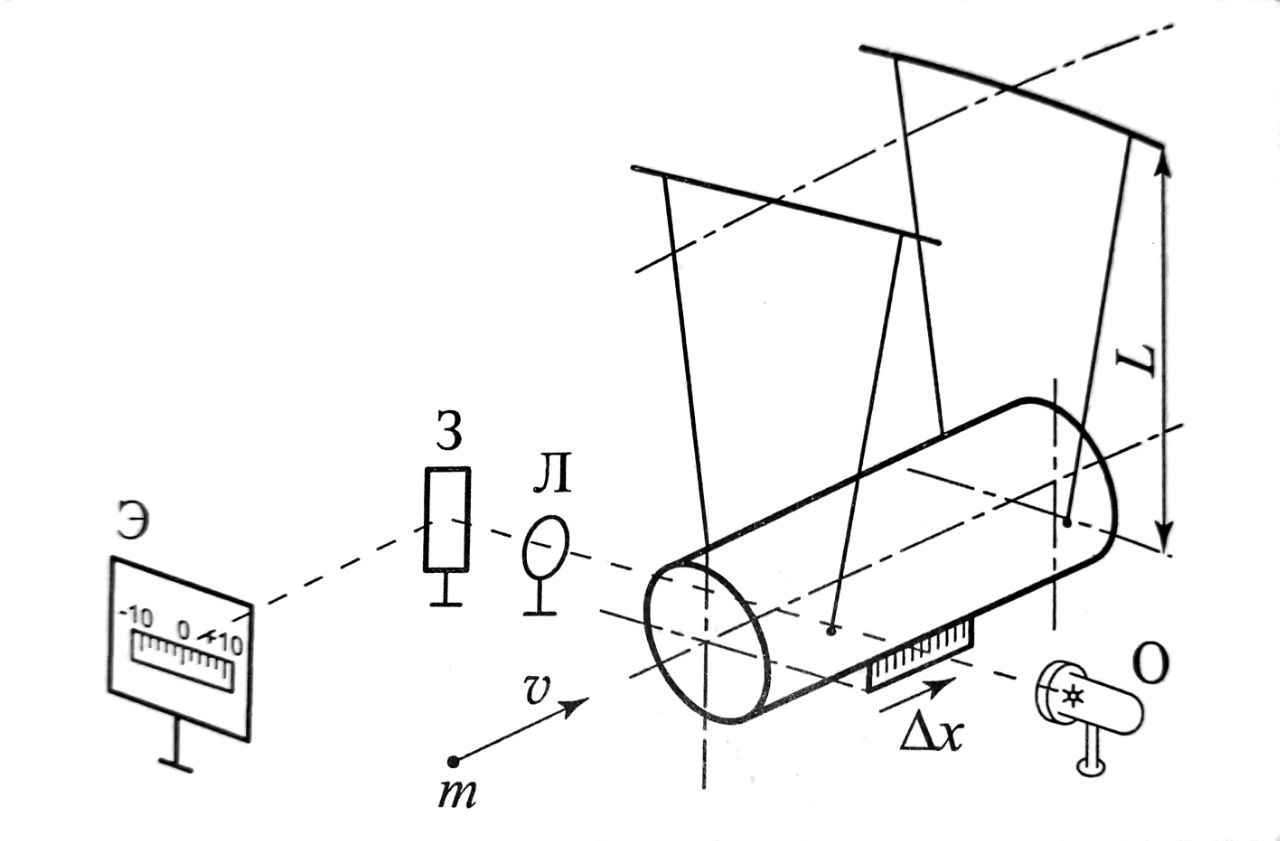
\includegraphics[width=0.7\linewidth]{ball}
		\caption{Схема установки для измерения скорости полета пули}
		\label{fig:ball}
	\end{figure}
	
	При взаимодействии маятника и пули можно считать импульс постоянным, так как время взаимодействия сильно меньше периода колебаний маятника. Следовательно отклонение от положения равновесия за время взаимодействия много меньше амплитуды колебаний.\\
	
	Закон сохранения импульса:
	\begin{equation}
		\label{pconst}
		mu=(M+m)v_0
	\end{equation}
	где $m$ -- масса пули, $M$ -- масса маятника, $u$ -- искомая скорость пули, $v_0$ -- начальная скорость системы маятник-пуля.\\	
	
	Учитывая, что масса пули много меньше массы маятника, можно сказать что
	\begin{equation}
		\label{u}
		u=\frac{M}{m}v_0
	\end{equation}
	
	Далее, так как колебания маятника слабо затухающие, можно считать, что энергия в первые несколько колебаний сохраняется. Отсюда, зная массу маятника и пули, а также амплитуду колебаний, мы можем узнать начальную скорость маятника, а значит узнать и скорость пули до взаимодействия.\\	
	
	Закон сохранения энергии:
	\begin{equation}
		\label{Econst}
		(M+m)v_0^2=(M+m)gh
	\end{equation}
	где $h$ -- подъем маятника, $g$ -- ускорение свободного падения.\\
	
	Высоту подъема маятника можно вывести через угловую амплитуду:
	\begin{equation}
		\label{h}
		h=L(1-\cos\varphi)=2L\sin^2\frac{\varphi}{2}
	\end{equation}
	где L -- высота подвеса. Учитывая что $\varphi$ -- мал, его можно выразить как
	\begin{equation}
		\label{varphi}
		\varphi\approx\frac{\Delta x}{L}
	\end{equation}
	Из соотношений \eqref{u}, \eqref{Econst}, \eqref{h} получим конечную формулу для скорости пули $u$:
	\begin{equation}
		\label{ufinal}
		u=\frac{M}{m}\sqrt{\frac{g}{L}}\Delta x
	\end{equation}
	
	\subsection{Метод крутильного маятника}
	
	\begin{figure}[H]
		\centering
		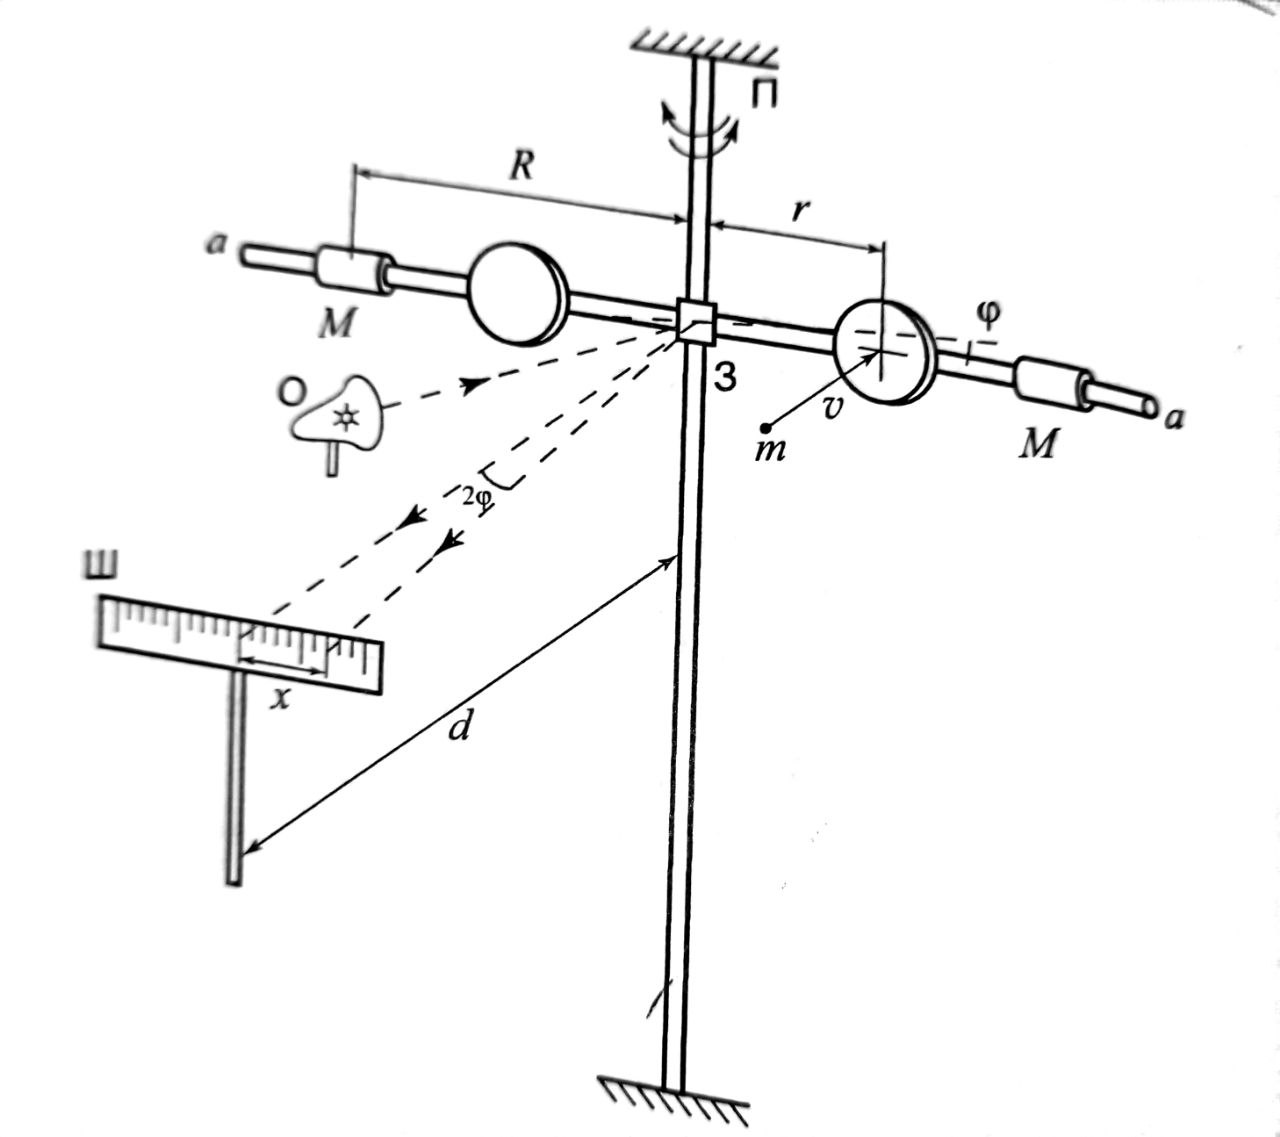
\includegraphics[width=0.7\linewidth]{rot}
		\caption{Схема установки крутильного маятника}
		\label{fig:rot}
	\end{figure}
	
	Относительно оси маятника можно записать закон сохранения момента импульса:
	\begin{equation}
		\label{Lconst}
		mru=I\omega_0
	\end{equation}
	где $r$ -- расстояние от оси маятника до места попадания пули, $\omega_0$ -- начальная угловая скорость маятника.\\
	
	Далее, в процессе движения маятника его энергия вращения переходит в упругую энергию закручивания проволоки. Колебания достаточно слабо затухающие, что мы можем считать энергию постоянной в течение нескольких первых колебаний.\\
	
	Закон сохранения энергии:
	\begin{equation}
		\label{Econst2}
		k\frac{\varphi^2}{2}=I\frac{\omega_0^2}{2}
	\end{equation}
	где $k$ -- модуль кручения проволоки $\Pi$, $\varphi$ -- максимальный угол поворота маятника.\\
	
	Из уравнений \eqref{Lconst}, \eqref{Econst2} получим
	\begin{equation}
		\label{ufinal2}
		u=\varphi\frac{\sqrt{kI}}{mr}
	\end{equation}
	
	\paragraph{Методика измерения $\varphi$ и момента инерции $I$} Стрельба производилась в маятник без дополнительных грузов. Чтобы найти момент инерции маятника в такой конфигурации необходимо найти период собственных колебаний $T_1$, а затем, поменяв конфигурацию на известный дополнительный момент инерции $\Delta I$ и измерив период $T_2$, можем найти изначальный момент инерции $I$.\\
	
	Угол максимального отклонения находится с помощью лазерной линейки. Измерив отклонение точки лазера на этой линейке и расстояние от нее до оси маятника, мы можем найти малый угол $\varphi$
	
	\begin{equation}
		\label{varphi2}
		\varphi\approx\frac{x}{d}
	\end{equation}
	где $d$ -- расстояние от оси маятника до линейки.\\
	
	Уравнения для момента инерции:
	
	\begin{equation}
		\label{T1}
		T_1=2\pi\sqrt{\frac{I}{k}}
	\end{equation}
	
	\begin{equation}
		\label{T2}
		T_2=2\pi\sqrt{\frac{I+2MR^2}{k}}
	\end{equation}
	
	Тогда величина $\sqrt{kI}$ находится следующим образом:
	\begin{equation}
		\label{kI}
		\sqrt{kI}=\frac{4\pi MR^2 T_1}{T_2^2-T_1^2}
	\end{equation}
	
	где $R$ -- расстояние от оси до дополнительных грузов, $M$ - масса этих грузов.
	
	\section{Результаты измерений и их обработка}
	
	\paragraph{Измерение масс пуль}
	
	В работе нам было предоставлено 10 пронумерованных пуль, 1-5 были использованы для баллистического маятника, а 6-10 для крутильного. Масса каждой пули была измерена на 3х разных весах, что позволило определить точность измерения\\
	
	\begin{table}[H]
		\centering
		\begin{tabular}{|c|c|c|c|c|}
			\hline
			& 1 & 2 & 3 & $\sigma_m$ \\
			\hline
			$m_1$ & 0.503 & 0.508 & 0.505 & 0.002 \\
			\hline
			$m_2$ & 0.499 & 0.502 & 0.500 & 0.002 \\
			\hline
			$m_3$ & 0.510 & 0.511 & 0.511 & 0.001 \\
			\hline
			$m_4$ & 0.503 & 0.503 & 0.504 & 0.001 \\
			\hline
			$m_5$ & 0.507 & 0.508 & 0.508 & 0.001 \\
			\hline
			$m_6$ & 0.502 & 0.501 & 0.503 & 0.001 \\
			\hline
			$m_7$ & 0.497 & 0.498 & 0.498 & 0.001 \\
			\hline
			$m_8$ & 0.498 & 0.499 & 0.500 & 0.001 \\
			\hline
			$m_9$ & 0.508 & 0.510 & 0.510 & 0.001 \\
			\hline
			$m_{10}$ & 0.516 & 0.517 & 0.518 & 0.001 \\
			\hline
		\end{tabular}
		\caption{Результаты измерений масс пуль}
	\end{table}	
	
	\subsection{Баллистический маятник}
	
	Масса маятника была известна заранее и равна $M=2900\pm5$ g. Высота подвеса $L=223.5\pm1.0$ cm.\\
	
	\begin{table}[H]
		\centering
		\begin{tabular}{|c|c|}
			\hline
			Пуля & $\Delta x$, mm \\
			\hline
			1 & 12.75 \\
			\hline
			2 & 12.00 \\
			\hline
			3 & 12.75 \\
			\hline
			4 & 12.00 \\
			\hline
			5 & 11.75 \\
			\hline
		\end{tabular}
		\caption{Результаты амплитуды колебаний баллистического маятника}
	\end{table}
	
	Полную погрешность результата будем рассчитывать по формуле:
	
	\begin{equation}
		\label{sigmax1}
		\sigma_x=\sqrt{\sigma_{rnd}^2+\sigma_{sys}^2}
	\end{equation}
	Системной погрешностью будем считать цену деления $\sigma_{sys}=0.25$ mm.\\
	
	Тогда погрешность измерений $\sigma_x = 0.53$ mm\\
	
	По формуле \eqref{ufinal} находим $u$, погрешность $\sigma_u$ вычисляем по формуле:
	\begin{equation}
		\label{sigmau1}
		\sigma_u = u\sqrt{\left(\frac{\sigma_m}{m}\right)^2+\left(\frac{\sigma_M}{M}\right)^2+\left(\frac{1}{2}\frac{\sigma_
				L}{L}\right)^2+\left(\frac{\sigma_x}{\Delta x}\right)^2}
	\end{equation}
	
	\begin{table}[H]
		\centering
		\begin{tabular}{|c|c|c|c|c|c|}
			\hline
			Пуля & 1 & 2 & 3 & 4 & 5 \\
			\hline
			$u$, m/s & 153.34 & 145.76 & 151.74 & 144.89 & 140.66 \\
			\hline
			$\sigma_u$ & 6.44 & 6.47 & 6.33 & 6.42 & 6.36 \\
			\hline
		\end{tabular}
		\caption{Полученные скорости пуль}
	\end{table}
	
	Тогда по формуле:
	
	\begin{equation}
		\label{chisigma}
		\sigma_u=\left(\sum_{i=1}^{5}\frac{1}{\sigma_i^2}\right)^{-1/2}
	\end{equation}
	
	\begin{center}
		\fbox{$u=147.28\pm2.53$ m/s}
	\end{center}
	
	
	\subsection{Крутильный маятник}
	
	Массы дополнительных грузов $m_1=730.6\pm 0.1$ g, $m_2=713.4\pm 0.1$ g.\\
	
	\begin{table}[H]
		\centering
		\begin{tabular}{|c|c|}
			\hline
			Пуля & $\Delta x$, cm \\
			\hline
			6 & 5.9 \\
			\hline
			7 & 5.6 \\
			\hline
			8 & 6.1 \\
			\hline
			9 & 5.7 \\
			\hline
			10 & 6.1 \\
			\hline
		\end{tabular}
	\end{table}
	
	Полную погрешность, аналогично баллистическому маятнику будем рассчитывать по формуле \eqref{sigmax1}, цена деления 0.1 cm\\
	
	Тогда полная погрешность $\sigma_x\approx0.25$ cm.\\
	
	\paragraph{Измерение момента инерции $I$}
	Для того, чтобы найти момент инерции крутильного маятника, а точнее величину $\sqrt{kI}$, которая необходима для расчета скорости по формуле \eqref{ufinal2}, необходимо измерить период собственных колебаний маятника с моментами инерции $I$ и $I+\Delta I= \newline=I+m_1R^2+m_2R^2$.\\
	
	Измерения проводились по 5 полных колебаний, 3 раза для каждой конфигурации маятника:
	
	\begin{table}[H]
		\centering
		\begin{tabular}{|c|c|c|c|}
			\hline
			& 1 & 2 & 3\\
			\hline
			$T_1$, s & 6.434 & 6.314 & 6.346 \\
			\hline
			$T_2$, s & 4.720 & 4.766 & 4.670 \\
			\hline
		\end{tabular}
		\caption{Результаты измерений периода колебаний для двух конфигураций маятника}
	\end{table}
	
	Полную погрешность измерения периода $T$ вычисляем по формуле:
	
	\begin{equation}
		\label{sigmaT}
		\sigma_T=\sqrt{\sigma_{rnd}^2+\sigma_{sys}^2}
	\end{equation}
	за $\sigma_{sys}$ возьмем среднюю скорость реакции человека, поделенную на количество периодов (т.е $0.2/5$).\\
	
	Тогда $T_1=6.365\pm0.074$ s, $T_2=4.719\pm0.062$ s.\\
	
	Найдем величину $\sqrt{kI}$ по формуле \eqref{kI}. $R=32.5\pm0.5$ cm, $M=0.722$ kg (среднее двух грузов, так как $m_1+m_2=2M$)\\
	
	Погрешность $\sqrt{kI}$ (в единицах СИ) будем вычислять по формуле:
	
	\begin{equation}
		\label{sigmakI}
		\sigma_{\sqrt{kI}}=\sqrt{kI}\left(\left(\frac{\sigma_M}{M}\right)^2+\left(2\frac{\sigma_R}{R}\right)^2+ \left(3\frac{\sigma_{T_1}}{T_1}\right)^2+\left(2\frac{\sigma_{T_2}}{T_2}\right)^2\right)^{(1/4)}
	\end{equation}
	
	Погрешность угла $\varphi$ будем рассчитывать по формуле:
	
	\begin{equation}
		\label{sigmavarphi}
		\sigma_{\varphi}=\varphi \sqrt{\left(\frac{\sigma_x}{x}\right)^2+\left(\frac{\sigma_d}{d}\right)^2}
	\end{equation}
	
	А погрешность скорости пули $u$ по формуле:
	
	\begin{equation}
		\label{sigmau2}
		\sigma_u=u\sqrt{\left(\frac{\sigma_{\sqrt{kI}}}{\sqrt{kI}}\right)^2+\left(\frac{\sigma_{\varphi}}{\varphi}\right)^2+\left(\frac{\sigma_r}{r}\right)^2+\left(\frac{\sigma_m}{m}\right)^2}
	\end{equation}
	
	\begin{table}[H]
		\centering
		\begin{tabular}{|c|c|c|c|c|c|}
			\hline
			Пуля & 1 & 2 & 3 & 4 & 5 \\
			\hline
			$m$, g & 0.502 & 0.498 & 0.499 & 0.509 & 0.517 \\
			\hline
			$\sigma_m$, g & 0.001 & 0.001 & 0.001 & 0.001 & 0.001 \\
			\hline
			$x$, cm & 5.9 & 5.6 & 6.1 & 5.7 & 6.1 \\
			\hline
			$\varphi$, rad & 0.045 & 0.043 & 0.047 & 0.044 & 0.047 \\
			\hline
			$\sigma_\varphi$, rad & 0.002 & 0.002 & 0.002 & 0.002 & 0.002 \\
			\hline
			$\sqrt{kI}$, in SI & 0.334 & 0.334 & 0.334 & 0.334 & 0.334 \\
			\hline
			$\sigma{kI}$, in SI & 0.025 & 0.025 & 0.025 & 0.025 & 0.025 \\
			\hline
			$u$, m/s & 143.94 & 137.72 & 149.71 & 137.15 & 144.50 \\
			\hline
			$\sigma_u$, m/s & 12.97 & 12.55 & 13.39 & 12.45 & 12.92 \\
			\hline
		\end{tabular}
		\caption{Полученные скорости пуль}
	\end{table}
	
	Тогда по формуле \eqref{chisigma}:

	\begin{center}
		\fbox{$u=142.60\pm5.74 m/s$}
	\end{center}
	
	\section{Обсуждение результатов и выводы}
	В результате выполнения работы была получена скорость пули, выпущенной из пневматического оружия двумя способами: с помощью подвешенного баллистического маятника и с помощью крутильного баллистического маятника. Результаты хорошо соотносятся, однако в первом случае погрешность оказалась недооценена.\\
	
	Расхождение результатов также может быть объяснено разной скоростью выхода пули у первого ружья и у второго ружья и ли большим влиянием внешних сил (таких как трение или сопротивление воздуха) на второй маятник.
	
	
	
\end{document}